\input{./econtexRoot.texinput}
\documentclass[\econtexRoot/HAFiscal]{subfiles}
\onlyinsubfile{\externaldocument{\econtexRoot/HAFiscal}} % Get xrefs -- esp to apndx -- from main file; only works if main file has already been compiled

\begin{document}

\FloatBarrier
\hypertarget{robustness}{}\par\section{Robustness}
\notinsubfile{\label{sec:robustness}}

In this section, we analyze how sensitive our results are to some of the parameters in the model. In particular, we focus on parameters that heavily influence consumers' incentives to save. These parameters are (1) the interest rate that affects the returns on saving and (2) the degree of risk aversion and the replacement rates when unemployed with or without benefits that affect the strength of a precautionary saving motive. The aim is to alter these incentives while maintaining the requirement that the distributions of liquid wealth in each education group match the distributions in the data. Hence, in each case, we re-estimate the distributions of discount factors in each education group (and, if necessary, the degree of splurge spending in consumption). The aim is thus to compute new results for a model with different parameters that also fits data on the distribution of liquid wealth. At the end of the section, we also consider how changing the properties of the recession affects our main results. 

\hypertarget{changing-the-interest-rate}{}\par\subsection{Changing the interest rate}
\notinsubfile{\label{sec:robust_R}} 
In our baseline calibration, the interest rate is set to $1$ percent per quarter. Here, we consider the effect on our results of increasing or decreasing this value. Changes to the U.S. interest rate do not affect the estimation of the splurge parameter $\varsigma$. However, before we can calculate updated results for a different interest rate, the distribution of discount factors within each education group must be re-estimated for the model to continue to match the liquid wealth distributions. 

\subsubsection{Discount factor distributions with different interest rates}
\notinsubfile{\label{sec:robust_R_estim}}

Table~\ref{tab:robustness_R} shows the values we obtain for the discount factor distributions when we change the quarterly interest rate by either decreasing it to $0.5$ percent or increasing it to $1.5$ percent. In both cases, the estimation can exactly match the median liquid-wealth-to-permanent-income ratios for each education group reported in panel~B of table~\ref{tab:estimBetas}. 

\begin{table}[t]
  \begin{center}
    \begin{tabular}{lc|cccccc} 
      \toprule
      & & \multicolumn{2}{c}{Dropout} & \multicolumn{2}{c}{Highschool} & \multicolumn{2}{c}{College} \\ \midrule 
      & Splurge & $\beta$ & $\nabla$ & $\beta$ & $\nabla$ & $\beta$ & $\nabla$ \\ \midrule 
      $R = 1.005$ & 0.307 & 0.701 & 0.520 & 0.909 & 0.099 & 0.983 & 0.014 \\
      $R = 1.01$ (baseline) & 0.307 & 0.694 & 0.542 & 0.904 & 0.099 & 0.978 & 0.015 \\ 
      $R = 1.015$ & 0.307 & 0.691 & 0.542 & 0.899 & 0.099 & 0.973 & 0.016 
      \\ \bottomrule 
    \end{tabular}
    \caption{Estimates of the splurge and $(\beta,\nabla)$ for each education group for different values of the interest rate $R$}
    \notinsubfile{\label{tab:robustness_R}}
  \end{center}
\end{table}

The first row of table~\ref{tab:robustness_R} shows the estimated $\beta_e$ and $\nabla_e$ for the lower interest rate of $0.5$ percent per quarter. With a lower interest rate and an unchanged discount factor distribution, consumers would tend to substitute away from saving and toward current consumption. They would therefore accumulate less wealth, leading to a lower median liquid-wealth-to-permanent-income ratio. In all education groups, we therefore see that the estimated discount factor distributions are centered around higher values of $\beta$ to ensure that the model still matches the median liquid-wealth-to-permanent-income ratio in the data. An increase in patience cancels out the effect of the lower interest rate on median saving. Similarly, in the third row, we see the opposite effect when the interest rate is increased to $1.5$ percent. For Highschool and College consumers, the change in $R$ is almost exactly offset by the change in $\beta$.  

Figure~\ref{fig:LorenzPtsrobustnessR} in Appendix~\ref{app:DF_R} shows that the re-estimated model also matches the liquid wealth distributions for each of these values of the interest rate. From table~\ref{tab:robustness_R}, we see that the values of $\nabla_e$ for the three education groups do not need to change much for this to be the case. 

\FloatBarrier
\subsubsection{Results with different interest rates}
\notinsubfile{\label{sec:robust_R_results}}

In this section, we repeat the welfare analysis conducted in section \ref{sec:welfare} for different values of the interest rate. As in that section, the stimulus check and payroll tax cut policy have been adjusted to be of the same fiscal size as the UI extension. All three policies are implemented during a recession. We determine welfare results for the policies implemented both with and without aggregate demand effects.

As can be seen in table \ref{tab:robustness_R_results}, a higher interest rate increases the welfare benefits of all policies uniformly. This result is despite multipliers changing only very little with different interest rates.\footnote{The long-run multiplier of the policies increases by about 1 to 1.5 percent in moving from an interest rate of 1.01 (the baseline as reported in table \ref{tab:Multiplier}) to 1.015.} Higher interest rates result in higher welfare benefits, as measured in lifetime consumption units, for all policies because the benefits of the policies (in the numerator) are front-loaded compared with a proportional increase in consumption through all periods (in the denominator). Thus, increasing the interest rate---which is also the social planner's discount rate---reduces the value of a proportional increase in consumption by more than the consumption increases associated with each policy.  Nevertheless, the qualitative result that the extended UI benefits provide by far the highest welfare gains, followed by the stimulus checks, is strongly robust to changes in the interest rate.


\begin{table}[]
  \begin{center}
    \begin{tabular}{@{}lllll@{}}
      \toprule
      &                    & Stimulus check & UI extension & Tax cut \\ \cmidrule(l){1-5} 
      \multirow{3}{*}{no AD effects}            	& $R = 1.005$ 			& 0.005        & 0.283       & 0.001	\\
      & $R = 1.01$ (baseline) & 0.011        & 0.580       & 0.002   	\\
      & $R = 1.015$ 			& 0.016        & 0.888       & 0.002   	\\ \cmidrule(l){1-5}
      \multirow{3}{*}{AD effects}					& $R = 1.005$    		& 0.086        & 0.630       & 0.033  	\\		
      & $R = 1.01$ (baseline) & 0.171        & 1.266       & 0.065   	\\
      & $R = 1.015$    		& 0.254        & 1.905       & 0.098    \\ \cmidrule(l){1-5} 
    \end{tabular}
    \caption{Consumption-equivalent welfare gains in basis points, calculated for policies implemented in a recession with and without aggregate demand effects, for different values of the interest rate $R$}
    \notinsubfile{\label{tab:robustness_R_results}}
  \end{center}
\end{table}


\FloatBarrier
\hypertarget{changing-risk-aversion}{}\par\subsection{Changing risk aversion} 
\notinsubfile{\label{sec:robust_gamma}} 

In our baseline calibration, consumers have a risk aversion of $\gamma=2$, which is quite common in macroeconomic models. Here, we investigate how alternative values of $\gamma$ would influence our results. Again, we re-estimate the distribution of discount factors within each education group, but in this case, we also re-estimate the degree of splurge spending in consumption. 

\subsubsection{Discount factor distributions with different risk aversion}
\notinsubfile{\label{sec:robust_gamma_estim}}

Table~\ref{tab:robustness_gamma} displays the values we obtain for the splurge and the discount factor distributions when we change $\gamma$ to $1$ and $3$. The table shows that the splurge is not very sensitive to the degree of risk aversion. The splurge controls the degree of spending that consumers do before considering the trade off involved in optimally allocating spending over time and across different future states of the world. Risk aversion affects that trade off but does not have a big influence on a parameter that controls spending that is independent of that problem. 

\begin{table}[t]
  \begin{center}
    \begin{tabular}{lc|cccccc} 
      \toprule
      & & \multicolumn{2}{c}{Dropout} & \multicolumn{2}{c}{Highschool} & \multicolumn{2}{c}{College} \\ \midrule 
      & Splurge & $\beta$ & $\nabla$ & $\beta$ & $\nabla$ & $\beta$ & $\nabla$ \\ \midrule 
      $\gamma = 1.0$ & 0.314 & 0.671 & 0.464 & 0.948 & 0.121 & 0.992 & 0.017 \\ 
      $\gamma = 2.0$ (baseline) & 0.307 & 0.694 & 0.542 & 0.904 & 0.099 & 0.978 & 0.015 \\
      $\gamma = 3.0$ & 0.304 & 0.565 & 0.749 & 0.843 & 0.163 & 0.964 & 0.027 
      \\ \bottomrule 
    \end{tabular}
    \caption{Estimates of the splurge and $(\beta,\nabla)$ for each education group for different values of risk aversion, $\gamma$}
    \notinsubfile{\label{tab:robustness_gamma}}
  \end{center}
\end{table}

The second and third rows of table~\ref{tab:robustness_gamma} show results when we increase risk aversion from $\gamma=2.0$ to $\gamma=3.0$. Increasing risk aversion for all types within an education group makes the precautionary saving motive stronger for all consumers in that group. Ceteris paribus, these consumers would then increase the amount of liquid wealth they accumulate, and the median liquid-wealth-to-permanent-income ratio for the education group would increase. For all the education groups, the discount factor distributions are therefore centered around lower values of $\beta$ when risk aversion is increased to $3.0$. As for the increase in the interest rate in section~\ref{sec:robust_R_estim}, the decrease in patience counteracts the stronger incentive to save from the higher risk aversion. However, the reductions in $\beta$ when increasing risk aversion from $2.0$ to $3.0$ are much larger than when increasing the interest rate from $1$ to $1.5$ percent. 

The effects on $\nabla$ and the concentration of the liquid wealth distribution may be less intuitive. However, if the only changes were to increase risk aversion and to decrease $\beta$ while keeping $\nabla$ fixed at the value for $\gamma=2.0$, then the result would be a liquid wealth distribution that was much less concentrated than in the data. If all consumers in an education group are less patient, the reduction in saving is larger for the wealthier consumers. Thus, to maintain the concentrated wealth distribution, $\nabla$ increases substantially. The results are distributions of discount factors within each education group that are centered around lower values, but that are much more dispersed. The effect is that the discount factor for the most patient type within each education group is not changed very much, but the lowest discount factor is much lower than when $\gamma=2.0$, and the liquid wealth distributions remain as concentrated as they are in the data.\footnote{Note that as in the baseline case, the discount factor for the most patient type in the Dropout group is constrained by the GIC. When $\gamma=3.0$ a constraint is also binding for the least patient type in the Dropout group. The large value of $\nabla$ relative to $\beta$ would imply a negative discount factor, and to prevent this outcome we constrain the lowest discount factor to be $0.01$.}

When we decrease risk aversion to $\gamma=1.0$, however, we run into problems when estimating the discount factor distribution. Row~1 of table~\ref{tab:robustness_R} shows estimated parameters that give the model the best fit for the median liquid-wealth-to-permanent income ratios and the liquid wealth distributions for each education group. The results for the $\beta$ parameters reverse the intuition that we discussed for the case of $\gamma=3.0$. In this case, reducing risk aversion and the strength of the precautionary saving motive is counteracted by centering the discount factor distributions around higher values. To obtain the same amount of saving on average, consumers need to be more patient if they are less risk averse.  

\begin{table}[th]
  \begin{center}
    \begin{tabular}{lccc}
      \multicolumn{4}{l}{} \\ \midrule
      & Dropout & Highschool & College \\ \midrule
      Median LW/PI (data, percent) & 4.64 & 30.2 & 112.8 \\ 
      Median LW/PI (model, $\gamma = 1.0$, percent) & 0.00 & 30.1 & 112.8 \\	
      Median LW/PI (model, $\gamma = 2.0$, percent) & 4.64 & 30.2 & 112.8 \\
      Median LW/PI (model, $\gamma = 3.0$, percent) & 4.64 & 30.2 & 112.8 \\ \bottomrule
    \end{tabular}
    \caption{Median liquid-wealth-to-permanent-income ratios}
    \notinsubfile{\label{tab:robustness_gamma_mlwpi}}	
    \parbox{15cm}{\small \vspace{.05cm} \textbf{Note}: The table shows the weighted median ratio of liquid-wealth-to permanent-income from the 2004 SCF and in versions of the model with different risk aversion. In the annual data from the SCF, the annual PI is divided by 4 to obtain a quarterly number.\normalsize}
  \end{center}
\end{table}

Table~\ref{tab:robustness_gamma_mlwpi} shows that for $\gamma=1.0$, while the model can match the median liquid-wealth-to permanent-income ratios for the Highschool and College groups, it does not do so for the Dropout group. That said, figure~\ref{fig:LorenzPts_robustness_CRRA} shows the opposite results for matching the liquid wealth distribution within each education group: The model matches the distribution for the Dropout group, but not for the Highschool and College groups. 

\begin{figure}[th]
  \begin{center}
    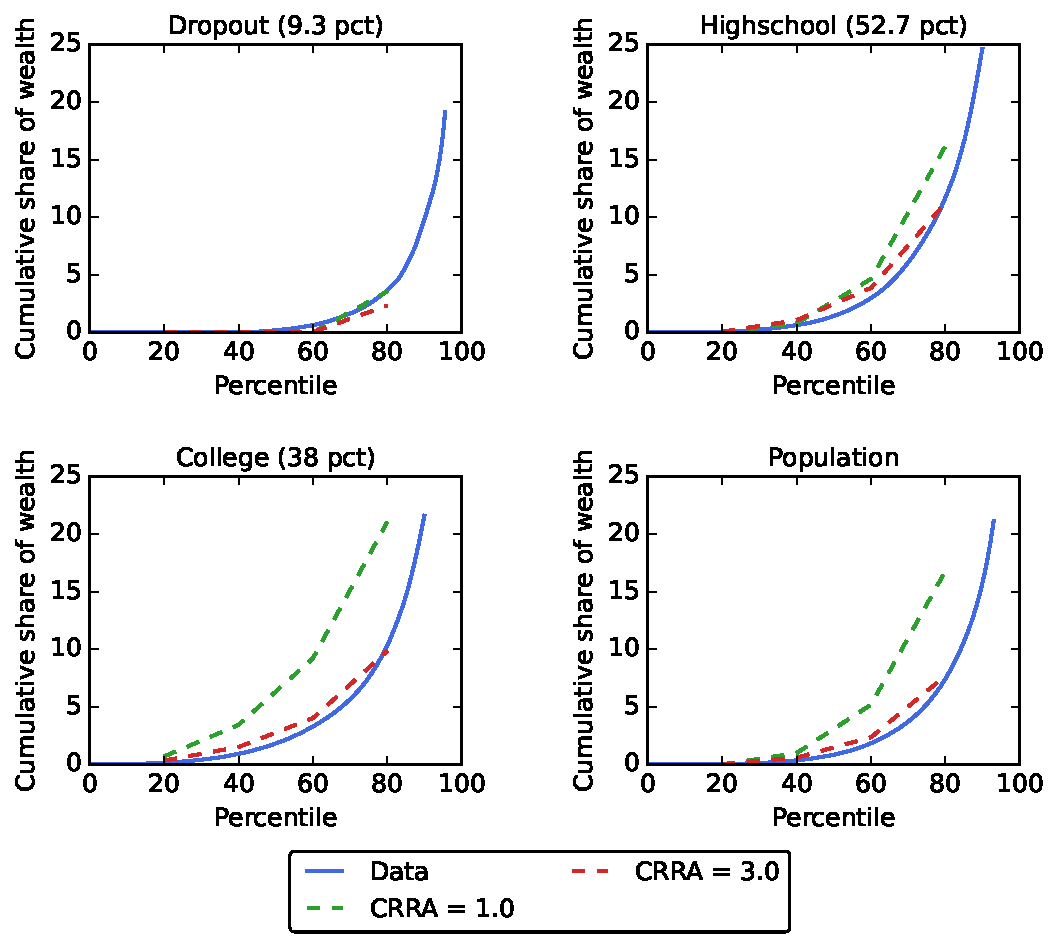
\includegraphics[width=.9\textwidth]{../Figures/LorenzPoints_robustness_CRRA.pdf}
    \caption{Distributions of liquid wealth within each educational group and for the whole population from the 2004 Survey of Consumer Finances and from the estimated model for different values of risk aversion, $\gamma$}
    \notinsubfile{\label{fig:LorenzPts_robustness_CRRA}}
  \end{center}
\end{figure}

The issue is that with a lower value of risk aversion and a weaker precautionary saving motive, the model requires consumers who are much more patient to obtain the same level and distribution of saving as in the baseline case with $\gamma=2.0$. In each education group the most patient types are then constrained by the GIC. When several types are constrained, then varying the estimated parameter values further may not improve on the fit of the model. Hence, the estimation terminates when hitting only one of the two targets. 

The strength of the precautionary saving motive, however, is determined by more than just risk aversion. The risks that households face also drive the strength of this motive for saving, and in our model, a key risk is unemployment risk. Therefore, the replacement rates that households face when they are unemployed with or without benefits play an important role. In section~\ref{sec:robust_benefits}, we consider an alternative calibration of these values. 

\subsubsection{Results with different risk aversion}
\notinsubfile{\label{sec:robust_gamma_results}}

In this section, we conduct the welfare analysis for different values of risk aversion. A higher risk aversion implies a greater welfare loss associated with the same drop in consumption, and thus, a greater welfare gain for policies that reduce the consumption drop. However, changing the risk-aversion parameter has a number of other ramifications for our welfare measure that are difficult to assess without simulation. A higher risk aversion (ceteris paribus) induces agents to hold a higher buffer stock of savings, making them less sensitive to adverse economic shocks in terms of their consumption response. As argued earlier, and since we target the empirical wealth-to-income ratios, we increase impatience to counteract this larger incentive to save. These changes then affect the consumption response of agents to the recession and to the policies implemented. 

Table \ref{tab:robustness_gamma_results} shows the welfare results for different risk-aversion parameters. The values for $\gamma = 1$ are difficult to interpret, given our difficulties in exactly matching the wealth distribution, as described in the previous section. Nevertheless, it is quite clear that despite the resulting imprecision, our ranking of the three policies is upheld also for $\gamma=1$.

For $\gamma=3$ and AD effects switched on, we obtain slightly higher welfare effects than in the baseline. When AD effects are switched off, there is either no change to the welfare results or a slight reduction as in the case of the UI extension. For both cases, with and without AD effects, the changes are quite small in magnitude.\footnote{Mirroring the welfare results, the long-run multipliers of the policies for the alternative risk aversion values are very close to those for the baseline calibration. The largest difference amounts to only a 3 percent increase in the multiplier for the UI extension policy in the $\gamma = 1$ case relative to the baseline.} Most importantly, the welfare ranking of the policies is fully robust to alternative values of the risk-aversion parameter.


\begin{table}[]
  \begin{center}
    \begin{tabular}{@{}lllll@{}}
      \toprule
      &                    & Stimulus check & UI extension & Tax cut \\ \cmidrule(l){1-5} 
      \multirow{3}{*}{no AD effects}            	& $\gamma = 1.0$ 			& 0.011          & 0.694        & 0.001   \\
      & $\gamma = 2.0$ (baseline) & 0.011          & 0.580        & 0.002   \\
      & $\gamma = 3.0$ 			& 0.011          & 0.577        & 0.002   \\ \cmidrule(l){1-5} 
      \multirow{3}{*}{AD effects}					& $\gamma = 1.0$   	 		& 0.182          & 1.378        & 0.067   \\
      & $\gamma = 2.0$ (baseline) & 0.171          & 1.266        & 0.065   \\
      & $\gamma = 3.0$    		& 0.172          & 1.273        & 0.066   \\ \cmidrule(l){1-5} 
    \end{tabular}
    \caption{Consumption-equivalent welfare gains in basis points, calculated for policies implemented in a recession with and without aggregate demand effects, for different values of risk aversion, $\gamma$}
    \notinsubfile{\label{tab:robustness_gamma_results}}
  \end{center}
\end{table}



\hypertarget{changing-benefits}{}\subsection{Changing benefits} 
\notinsubfile{\label{sec:robust_benefits}} 

In our baseline calibration, we follow \cite{rothstein2017scraping} and calibrate the replacement rates to $\rho_b=0.7$ with unemployment benefits and $\rho_{nb}=0.5$ without benefits. Here, we consider replacement rates that are considerably less generous and more in line with values used in the previous macro literature with unemployment in models with heterogeneous agents. The alternative values we consider are a replacement rate of $\rho_{b}=0.3$ when unemployed with benefits, as in \cite{carroll2020modeling}, and a replacement rate of $\rho_{nb}=0.15$ when unemployed without benefits. This latter value is the same as the replacement rate used in \cite{den2010computational}.\footnote{In \cite{den2010computational}, there is only one unemployment state and, hence, no sense in which benefits expire after a while. Therefore, this replacement rate applies for long-term unemployed, as it does in our model, but in this paper there is also an intermediate state in which benefits are higher until they expire.} With these replacement rates, being unemployed is more serious for consumers than in our baseline calibration, and the precautionary saving motive is stronger. 

\subsubsection{Discount factor distributions with different benefits}
\notinsubfile{\label{sec:robust_benefits_estim}}

Table~\ref{tab:robustness_benefits} shows that when benefits are less generous and the precautionary motive is stronger, the estimated discount factor distributions are centered on lower values of $\beta$, and the dispersion in the distributions increases, as $\nabla$ is considerably higher. The intuition is similar to the case when increasing risk aversion from $\gamma=2.0$ to $\gamma=3.0$, discussed in section~\ref{sec:robust_gamma_estim}: A stronger precautionary motive for saving must be counteracted by a lower average discount factor to match the same average level of saving as before. The distributions must also be more dispersed to match the same concentration of liquid wealth. In fact, the estimated discount factor distributions for the alternative calibration of the replacement rates are very similar to those reported for $\gamma=3.0$ in row~3 of table~\ref{tab:robustness_gamma}. 

\begin{table}[t]
  \begin{center}
    \begin{tabular}{llc|cccccc} 
      \toprule
      & & & \multicolumn{2}{c}{Dropout} & \multicolumn{2}{c}{Highschool} & \multicolumn{2}{c}{College} \\ \midrule 
      & & Splurge & $\beta$ & $\nabla$ & $\beta$ & $\nabla$ & $\beta$ & $\nabla$ \\ \midrule 
      Baseline & ($\rho_{b}=0.7$, $\rho_{nb}=0.5$) & 0.307 & 0.694 & 0.542 & 0.904 & 0.099 & 0.978 & 0.015 \\ 
      Altern. & ($\rho_{b}=0.3$,  $\rho_{nb}=0.15$) & 0.307 & 0.599 & 0.687 & 0.852 & 0.159 & 0.968 & 0.028
      \\ \bottomrule 
    \end{tabular}
  \end{center}
  \caption{Estimates of the Splurge and $(\beta,\nabla)$ for each education group for the baseline replacement rates $\rho_{b}$ and $\rho_{nb}$ and an alternative calibration}
  \notinsubfile{\label{tab:robustness_benefits}}
\end{table}


\FloatBarrier
\subsubsection{Results with different benefits}
\notinsubfile{\label{sec:robust_benefits_results}}

In this section, we perform the welfare analysis for different benefit replacement rates. Table \ref{tab:robustness_benefit_results} shows that the alternative parameterization of the unemployment replacement rates yields considerably higher welfare benefits for the UI extension policy. In particular, the lower the replacement rate under the no-benefit regime, the more harmful is the expiration of eligibility to the UI. The UI extension is thus particularly powerful if $\rho_{nb}$ is small, which is mirrored by the long-run multiplier of the UI extension policy. It increases from 1.275 in the baseline calibration to 1.416 under the lower replacement rates. In contrast, multipliers and welfare effects of the other two policies do not change dramatically under the alternative calibration. Again, our ranking of the three policies remains the same.


\begin{table}[]
  \begin{center}
    \begin{tabular}{@{}lllll@{}}
      \toprule
      &                    & Stimulus check & UI extension & Tax cut \\ \cmidrule(l){1-5} 
      \multirow{2}{*}{no AD effects} 	& Baseline  ($\rho_{b}=0.7$, $\rho_{nb}=0.5$) 		& 0.011          & 0.580        & 0.002   \\
      & Altern.  ($\rho_{b}=0.3$, $\rho_{nb}=0.15$) 	& 0.043          & 1.913        & 0.003   \\ \cmidrule(l){1-5} 
      \multirow{2}{*}{AD effects}		& Baseline  ($\rho_{b}=0.7$, $\rho_{nb}=0.5$)    	& 0.171          & 1.266        & 0.065   \\
      & Altern.  ($\rho_{b}=0.3$, $\rho_{nb}=0.15$)    & 0.169          & 2.620        & 0.052   \\ \cmidrule(l){1-5} 
    \end{tabular}
    \caption{Consumption equivalent welfare gains in basis points, calculated for policies implemented in a recession with and without aggregate demand effects, for different unemployment benefit rates}
    \notinsubfile{\label{tab:robustness_benefit_results}}
  \end{center}
\end{table}




\FloatBarrier
\hypertarget{changing-the-properties-of-the-recession}{}\par\subsection{Changing the properties of the recession}

In this section, we alter two properties of the recession and study the effect of those changes (one at a time) on our main results. First, we lower the average length of a recession from six quarters in the baseline to four quarters. Second, we increase the consumption elasticity of the aggregate demand effect, $\kappa$, from 0.3 in the baseline to 0.5. In either case, the parameter changes do not require a re-estimation of the discount factor distribution, since the baseline saving behavior is unaffected by properties of the recession, which arrives as an MIT shock. 

Table \ref{tab:robustness_recession_property_results} presents the welfare results for different properties of the recession. In case of a shorter average recession length of four quarters, as opposed to six quarters, in the baseline, we observe lower welfare effects of the policies. As argued earlier, the reason is that the policies are particularly effective during recessions. Hence, the additional spending induced by the policies is now less likely to occur while the recession is ongoing. This outcome can also be seen by investigating the long-run multipliers of the policies, which fall slightly for all three policies considered: from 1.339 in the baseline to 1.314 in case of the shorter recession length for the stimulus check, from 1.275 to 1.255 for the UI extension, and from 1.079 to 1.042 for the tax cut.

A higher value for $\kappa$---and hence stronger aggregate demand effects---considerably increases the welfare effects of each policy. Of course, this is only the case in the version of the model with aggregate demand effects. In their absence, there is no change in the welfare results relative to the baseline calibration of the model. The larger $\kappa$ implies a larger boost to aggregate income in response to the demand effects of the policies. This larger boost translates to a larger increase in consumption and thus a stronger welfare effect. Under stronger AD effects, the policies have also considerably larger long-run multipliers. The stimulus check exhibits a multiplier of 1.811 (baseline: 1.339); the UI extension, a multiplier of 1.633 (1.275); and the tax cut, a multiplier of 1.271 (1.079).


\begin{table}[]
  \begin{center}
    \begin{tabular}{@{}lllll@{}}
      \toprule
      &                    											& Stimulus check & UI extension & Tax cut 	\\ \cmidrule(l){1-5}
      \multirow{2}{*}{no AD effects} 					& Baseline 						& 0.011          & 0.580        & 0.002   	\\ 
      & Shorter average recession, 4q & 0.010          & 0.488        & 0.001  	\\
      & Stronger AD effects, 0.5 		& 0.011          & 0.580        & 0.002   	\\ \cmidrule(l){1-5}
      \multirow{2}{*}{AD effects}						& Baseline    					& 0.171          & 1.266        & 0.065   	\\
      & Shorter average recession, 4q & 0.161          & 1.074        & 0.053   	\\
      & Stronger AD effects, 0.5    	& 0.346          & 1.990        & 0.133   	\\ \cmidrule(l){1-5} 
    \end{tabular}
    \caption{Consumption-equivalent welfare gains in basis points, calculated for policies implemented in a recession with and without aggregate demand effects, for different properties of the recession}
    \notinsubfile{\label{tab:robustness_recession_property_results}}
  \end{center}
\end{table}




\FloatBarrier
\hypertarget{summary-of-robustness-exercises}{}\par\subsection{Summary of robustness exercises}
\notinsubfile{\label{sec:robust_summary}}

The robustness checks in this section show that our main results are fairly robust to a wide range of alternative parameter choices. We have shown that the ex-ante discount rates can be adjusted so that the distribution of liquid wealth is well approximated in the model. Furthermore, the distribution of liquid wealth appears to more or less pin down the aggregate consumption properties for the model, regardless of the other parameters. Importantly, none of the robustness checks alter the ranking of policies in terms of their effectiveness and therefore the overall conclusions of this paper.

Characteristics of the recession do, however, matter for our results. Shorter recessions or those with smaller aggregate demand effects reduce the effectiveness of policies. Conversely, more severe recessions will render the policies even more efficient than our baseline results suggest.

\ifthenelse{\boolean{Web}}{}{
  \end{document} \endinput
}
